\documentclass{hust}



\lfoot{Student Name - Student Id - Student Class}
\title{thesis}
\author{name}
\date{April 2021}
\usepackage{chngcntr}
\usepackage{mathptmx}
\usepackage{float}

\geometry{
top=2cm,
bottom=2cm,
left=3.5cm,
right=2.5cm,
headheight=17pt, % as per the warning by fancyhdr
includehead,includefoot,
heightrounded, % to avoid spurious underfull messages
}

%\usepackage{fancyhdr}
%\pagestyle{fancy}
%\fancyhf{}
%\renewcommand{\footrulewidth}{0pt}
%\fancyhead[LE,RO]{\leftmark}
%\fancyfoot[CE,CO]{\thepage}
%\makeglossaries
\loadglsentries{glossary}
\setcounter{tocdepth}{1}
\setcounter{tocdepth}{2}

\begin{document}
\thispagestyle{empty}
%
%\thisfancypage{
%  \setlength{\fboxrule}{1pt}
%  \doublebox}{}
\begin{center}

{\setstretch{1.4}
{\fontsize{14}{12}\selectfont \textbf{HANOI UNIVERSITY OF SCIENCE AND TECHNOLOGY}}\\
\textbf{---------------*******---------------}\\[1cm]

\includegraphics[width=3cm]{Figures/bklogo.jpg}
\centering
\\[1cm]
{\fontsize{25}{43}\selectfont \textbf{GRADUATION THESIS}}\\[0.3cm]
{\fontsize{22}{30}\selectfont \textbf{Thesis topic}}\\[0.3cm]
{\fontsize{14}{20}\selectfont \textbf{STUDENT NAME} \\
\fontsize{13}{18}\selectfont mail@sis.hust.edu.vn}\\[0.3cm]

{\fontsize{17}{10}\fontseries{b}\selectfont Major in ...}\\[1.5cm]

\vspace*{1\baselineskip}  
\begin{tabular}{l c l l}
  \textbf{Supervisor} & : &  Assoc. Prof. .... & \text{\_\_\_\_\_\_\_\_\_\_\_\_\_\_\_\_\_\_\_\_} \\
  & & & \fontsize{10}{10}\selectfont Signature of Supervisor\\
  \textbf{Department} & : &  .... \\
  \textbf{School} & : &  School of Information and Communication Technology \\
\end{tabular} \\[3cm]
}

\vspace*{1\baselineskip}  
\fontsize{15}{19}\selectfont \textbf{HA NOI, x/2021}
\end{center}
\pagebreak
\addcontentsline{toc}{chapter}{Graduation topic}
\chapter*{Requirements for the thesis}
\section*{Student information}

\begin{itemize}
\item \textbf{Student name:} Nguyen Hoang Long
\begin{multicols}{2}
\item \textbf{Tel:} 0969786349
\item \textbf{Class:} LTU16-K62
\item \textbf{Email:} long.nh176040@sis.hust.edu.vn
\item \textbf{Program:} Information Technology
\end{multicols}
\item \textbf{Graduation Thesis conducted:} From May 2022 to July 2022
%\item \textbf{Time:} xxx
\end{itemize}
\section*{Goal of the thesis}
\begin{enumerate}
	\item Research on \gls{idpcdu} as well as existing algorithms for this problem.
	\item Research on metaheuristic algorithms, especially \gls{ga} and \gls{aco}, and propose an effective strategy to solve \gls{idpcdu}.
\end{enumerate}

\section*{Main tasks}
\begin{enumerate}
	\item Survey \acrfull{idpcdu} and related studies.
	\item Propose a two-level algorithm combining \gls{ga} and an improved \gls{aco} to solve \gls{idpcdu}.
	\item Devise an anti-stuck strategy for ants when applying \gls{aco} to multi-domain network problems, such as \gls{idpcdu}.
	\item Conduct experiments on various test instances and comparison with several previous approaches to prove the efficiency of the proposed model.
\end{enumerate}

\pagebreak

\section*{Declaration of student}
I - Nguyen Hoang Long - hereby warrant that the Work and Presentation in this thesis are
performed by myself under the supervision of Mr. Do Tuan Anh.

All results presented in this thesis are truthful and are not copied from any other work.
\begin{minipage}{0.5\textwidth}
.
\end{minipage}
\begin{minipage}[t]{0.5\textwidth}



\begin{center}
  \textit{Ha Noi}, xx August 2022\\
  Author\\[3cm]
  
  \textit{Nguyen Hoang Long}
\end{center}
\end{minipage}
\subsection*{Attestation of the supervisor on the fulfillment of the requirements of the thesis}
.\dotfill \\
.\dotfill \\ 
.\dotfill \\ 
.\dotfill \\
\begin{minipage}{0.5\textwidth}
.
\end{minipage}
\begin{minipage}[t]{0.5\textwidth}

\begin{center}
  \textit{Ha Noi}, xx August 2022\\
  Supervisor\\[3cm]
  
  \textit{Mr. Do Tuan Anh}
\end{center}
\end{minipage}

\pagebreak

\begin{center}
	{\fontsize{14}{16}\selectfont\textbf{Acknowledgement}}
\end{center}



\begin{center}
	{\fontsize{14}{16}\selectfont \textbf{Abstract of thesis}}
\end{center}

For the past few years, \gls{hpce} is an architecture that has been promoted to handle packet routing in multi-domain networks. However, this architecture has a potential drawback of poor scalability with
respect to the number of domains. In tackling this complicated problem, \acrfull{idpcdu}, which is employed to improve h-PCE, is focused on this thesis. The objective of \gls{idpcdu} is to find the shortest path between two given nodes that traverses every domain at most once. Since the \gls{idpcdu} belongs to NP-Hard class, this thesis introduces a two-level approach, combining the advantages of two metaheuristic algorithms, \acrfull{ga} and \acrfull{aco}. Specifically, the upper-level \gls{ga} plays the role of navigating the path for ants at the lower level \gls{aco}. Furthermore, an anti-stuck strategy that helps ants avoid being stuck is also equipped. To analyze the effectiveness of the proposed algorithm, experiments and comparisons with other algorithms are conducted. The results demonstrated that the proposed algorithm outperforms all other compared ones in most cases.

\begin{flushright}
	\begin{minipage}[t]{0.5\textwidth}
		\begin{center}
			\textit{Ha Noi}, xx May 2022\\[2cm]
		
			\textit{Nguyen Hoang Long}
		\end{center}
	\end{minipage}
\end{flushright}
\pagebreak


\chapter*{Glossaries}
\addcontentsline{toc}{chapter}{Glossaries}
\fontsize{13}{16}
\fontfamily{ptm}\selectfont
%cmr
\begin{center}
	\begin{tabular}{|p{1in}|p{5in}|}
		\hline
		\textbf{Acronym} & \textbf{Meaning}  \\ \hline
		PCE & Path Computation Element	\\ \hline
		h-PCE & Hierarchical Path Computation Element	\\ \hline
		IDPC-DU & Inter-domain Path Computation problem under the Domain Uniqueness constraint \\ \hline
		IDPC-NDU & Inter-domain Path Computation problem under the Node-defined Domain Uniqueness constraint \\ \hline
		IDPC-EDU & Inter-domain Path Computation problem under the Edge-defined Domain Uniqueness constraint \\ \hline
		EA & Evolutionary Algorithm \\ \hline
		GA & Genetic Algorithm  \\ \hline
		ACO & Ant Colony Optimization \\ \hline
		AS & Ant System \\ \hline
		MFEA & Multifactorial Evolutionary Algorithm \\ \hline
		SBX & Simulated Binary Crossover\\ \hline
		PM & Polynomial Mutation\\ \hline
		RPD & Relative Percentage Difference\\ \hline
		PI & Improvement Percentage\\ \hline
	\end{tabular}    
\end{center}


\pagebreak


\listoftables
\addcontentsline{toc}{chapter}{List of Tables}
\listoffigures
\addcontentsline{toc}{chapter}{List of Figures}

\newpage
\tableofcontents
\newpage


%\acresetall

\chapter*{Preface}
\addcontentsline{toc}{chapter}{Preface}
Researching into graph problems has long attracted significant interest from the science community since numerous real-world problems can be modeled as graphs, such as transport services, logistics, and agricultural irrigation systems. Especially to meet the current surge in Internet usage, network optimization problems are typically prioritized to be solved. Stems from this practical the \gls{idpcdu}, which concentrates on handling the routing problem on multi-domain networks. 

\gls{idpcdu} takes the context of the \gls{hpce} architecture, in which a parent \gls{pce} performs inter-domain path computation based on the gathered intra-domain routing information from its children PCEs~\cite{paolucci2013survey}. By integrating the optimal order of crossed domains with path computation, the \gls{hpce} can effortlessly achieve the packet's route optimality. However, as the number of domains grows, this architecture is regarded as infeasible due to the existence of two bottlenecks, namely the parent \gls{pce}'s processing capabilities and the capacity of the Children-to-Parent \gls{pce} communication channel~\cite{king2012application}. \gls{idpcdu} thus introduces a viable condition, called the \gls{du}, to overcome the inherent problem of packet processing delays in \gls{hpce} when being applied to large-scale networks, that is, preventing a path from visiting a domain more than once. In particular, each path found by \gls{idpcdu} must be the shortest one between two fixed nodes, possibly belong to the same or different network domains, and satisfy the above constraint. Consequently, \gls{idpcdu} has been proven to be in the NP-Complete class~\cite{maggi2018domain}. 

In light of \gls{idpcdu}'s complexity, metaheuristic algorithms are proper techniques to tackle this problem. \gls{ga} and \gls{aco} are some example algorithms that fall under this class. \gls{ga} is based on Darwin's Theory of Evolution, which holds that the better individuals are able to adapt to their surroundings, the better their chances of surviving and passing their traits to future generations. On the other hand, \gls{aco} simulates the natural foraging process of ants.

Accordingly, there have been several proposals to solve \gls{idpcdu} in the literature. However, these previous approaches are deemed ineffective because they often use only a single metaheuristic algorithm while the search space is massive with a considerable number of edges. For this reason, this thesis introduces a two-level strategy that combines the advantages of both \gls{ga} and \gls{aco} for \gls{idpcdu}. Particularly, the upper-level \gls{ga} plays the role of navigating the path for ants at the lower one. In addition, an anti-stuck method is integrated into the improved \gls{aco} algorithm, which helps to address the problem of ant being stuck when applying it to multi-domain network problems. This combination is expected to improve the quality of final solutions compared to the prior techniques.

The major contributions of this thesis can be summarized as follows:
\begin{itemize}
	\item Propose a two-level algorithm combining \gls{ga} and an improved \gls{aco} to solve \gls{idpcdu}.
	\item Devise an anti-stuck strategy for ants when applying \gls{aco} to multi-domain network problems, such as \gls{idpcdu}.
	\item Conduct experiments on various test instances and comparison with several previous approaches to prove the efficiency of the proposed model.
\end{itemize}

This thesis consists of 4 chapters as follows:
\begin{itemize}
	\item \textbf{Chapter 1:} Overview current popular approximate and approximation algorithms, especially Genetic Algorithm and Ant Colony Optimization.
	\item \textbf{Chapter 2:} Introduce to the Inter-domain Path Computation problem under the Domain Uniqueness constraint. This chapter also presents the problem statement and its related works.
	\item \textbf{Chapter 3:} Elaborate on the proposed algorithm, including detailed descriptions of each of its components.
	\item \textbf{Chapter 4:} Includes the experimental setups, computational results on various test sets, and a performance comparison with other algorithms
\end{itemize}



\chapter{Theoretical background}
\label{chap:chap1}

\chapter{The problem}
\label{chap:chap2}

\chapter{A Genetic Ant Colony Optimization Algorithm for Inter-domain Path Computation problem under the Domain Uniqueness constraint}
\label{chap:chap3}
This section introduces the proposed two-level genetic ant colony optimization algorithm, called \acrshort{gaco} hereafter, to solve \gls{idpcdu} in more detail. Each level in \acrshort{gaco} is responsible for a separate task, where the first level establishes the domains' priorities, which are then used as input for the second one to find the final solution. The structure of \acrshort{gaco} is presented in Figure~\ref{fig:flowchart}.

\setlength{\intextsep}{3pt}
\renewcommand{\scalefigure}{0.85}
\begin{figure}[htbp]
	\centering
	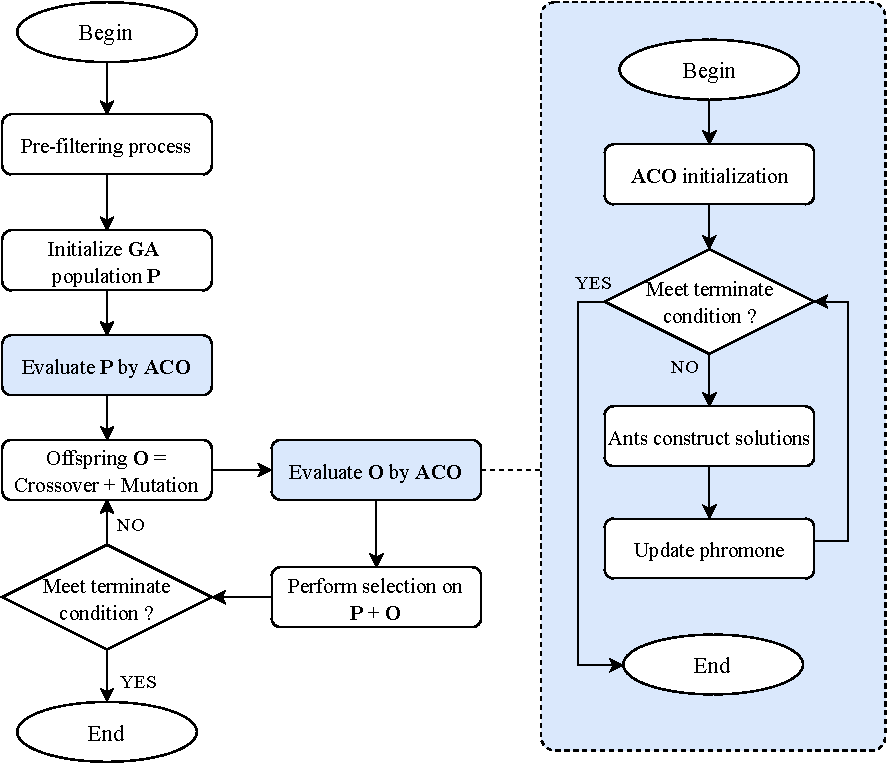
\includegraphics[scale=\scalefigure]{Figures/chap 3/Flowchart.pdf}
	\caption{The structure of \acrshort{gaco}}
	\label{fig:flowchart}
\end{figure}

\section{Pre-filtering Process}
\label{proposed:prefiltering}
Clearly, \gls{idpcdu}'s primary goal is to locate the minimally costly path. Therefore, to accelerate the search process and reduce resource consumption as well as computation time, a pre-filtering process, based on~\cite{binh2021two}, is applied to the input graph $G$ as follows. Firstly, we prune all edges that enter the source node $s$ and leave the target node $t$. Secondly, let $D^k_{i,j}$ be the set of $k$-colored edges going from node $i$ to $j$. If the length of $D^k_{i,j}$ is greater than one, we preserve only the lowest-weight edge and remove the remaining ones in $D^k_{i,j}$. Finally, apart from the source $s$ and target $t$, any node whose indegree and outdegree is 0, is likewise eliminated from $V$. Figure~\ref{fig:filtered_graph} demonstrates $G'=(E', V')$ as a result after performing the pre-filtering process on the input graph.

\setlength{\intextsep}{3pt}
\renewcommand{\scalefigure}{0.8}
\begin{figure}[htbp]
	\centering
	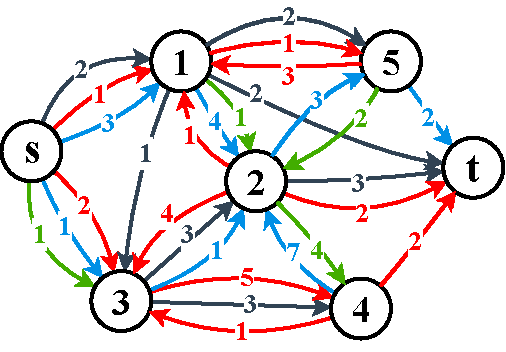
\includegraphics[scale=\scalefigure]{Figures/chap 3/Bold Filtered Graph.pdf}
	\caption{The filtered graph $G'$}
	\label{fig:filtered_graph}
\end{figure}

\section{Individual Representation}
\label{proposed:encoding}
This section introduces a scheme to represent a solution of \gls{idpcdu} as an individual in \gls{ea}. In general, for a difficult problem, significant advantages may be gained by an effective encoding method. Instead of conventional path encoding approach (such as representing a path from $s$ to $t$ with a list of edges/nodes between them), each chromosome is constructed by an array of real numbers whose length is equal to the number of domains. Each element, which denotes the priority of each domain, is randomly drawn between 0 and 1. The higher the priority value, the earlier the domain is likely to be visited. Each chromosome is then evaluated by an improved \gls{aco} algorithm, where the domain's priority will act as a factor influencing the ant's route selection. This encoding helps with facilitating the evolution operators by ensuring all chromosomes' length is equal. Furthermore, in many practical cases, the number of domains is remarkably smaller than the number of nodes or edges. 
Figure~\ref{fig:individual} delineates an example of an individual representation, in which the priority values of each domain are $red - 0.8$, $blue - 0.2$, $green - 0.6$, and $grey - 0.3$, respectively.
\setlength{\intextsep}{3pt}
\renewcommand{\scalefigure}{1.2}
\begin{figure}[htbp]
	\centering
	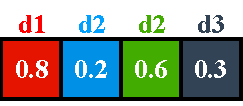
\includegraphics[scale=\scalefigure]{Figures/chap 3/Individual.pdf}
	\caption{A representation of a chromosome}
	\label{fig:individual}
\end{figure}

\section{Evolutionary Operators}
\label{proposed:operator}
\subsection{Crossover}
Since the proposed encoding utilizes an array of real numbers, this thesis apply the \gls{sbx}~\cite{deb1995simulated}. \gls{sbx} has been applied in many real-coded \gls{ga} problems and it also has proven to be effective. The implementation steps of \gls{sbx} can be summarized as follows. Firstly, choose a random number $u = [ \, 0, 1) \,$. Next, the ratio of the difference in offspring values to their parents' values $\beta$ is calculated as:
\begin{equation}
	\beta = 
	\begin{cases}
		(2u)^{\frac{1}{\eta_c + 1}}, & \text{if $u \leq 0.5$},\\
		(\frac{1}{2(1 - u)})^{\frac{1}{\eta_c + 1}}, & \text{otherwise},
	\end{cases}  
\end{equation}
where $\eta_c$ is any non-negative real number indicating the distribution index. A large value of $\eta_c$ increases the likelihood of generating near-parent solutions, whereas a small one allows for the selection of distant solutions as children. Finally, for two parents $p_1$ and $p_2$, two offspring $o_1$ and $o_2$ are reproduced using:
\begin{equation}
	o^i_1 = 0.5*[(1-\beta)*p^i_1 + (1+\beta)*p^i_2],
\end{equation}
\begin{equation}
	o^i_2 = 0.5*[(1+\beta)*p^i_1 + (1-\beta)*p^i_2].
\end{equation}

\subsection{Mutation}
In like manner, this thesis use \gls{pm}~\cite{deb2014analysing}, which is also an operator used in real-coded \gls{ga}. From a selected parent $p$, the \gls{pm} produces an individual $p'$ as follows. Similar to \gls{sbx}, a random number $u = 	[ \, 0, 1) \,$ is picked at first. For each element $p_i$, the $\delta_i$ is calculated as:
\begin{equation}
	\delta_i = 
	\begin{cases}
		(2u)^{\frac{1}{\eta_m + 1}} - 1, & \text{if $u \leq 0.5$},\\
		1 - [2(1-u)]^{\frac{1}{\eta_m + 1}}, & \text{otherwise},
	\end{cases}
\end{equation}
where $\eta_m$ is any non-negative real number indicating the polynomial distribution index. The perturbance can be varied in the mutated solution by changing $\eta_m$ value. $p'$ is then updated using the following equation:
\begin{equation}
	p' = 
	\begin{cases}
		p + \delta_i * p, & \text{if $u \leq 0.5$},\\
		p + \delta_i * (1-p), & \text{otherwise},
	\end{cases}
\end{equation}

\subsection{Selection}
Roulette Selection is used for selecting parents.

\section{Proposed Ant Colony Optimization as Fitness Evaluation}
\label{proposed:aco}
Corresponding to each chromosome, an improved \gls{aco} algorithm that plays the fitness evaluation role as well as finds the shortest path from the source node to the target node is proposed. 
To travel from node $v_i$, the $k^{th}$ ant must choose an edge $e$ in the $Adj(v_i)$ through a transition probability function (Equation~\ref{equation:edge_pick}).
\begin{equation}
	\label{equation:edge_pick}
	p_e(t) = 
	\frac{[\tau_e(t)]^{\alpha} \cdot [\eta_e(t)]^{\beta} \cdot  [P_e(t)]^{\gamma}}{\Sigma_{h \in Adj(v_i)} [\tau_h(t)]^{\alpha} \cdot [\eta_h(t)]^{\beta} \cdot [P_h(t)]^{\gamma}},
\end{equation}
where $P_e$ is the domain's priority of edge $e$ obtained from the input chromosome, and $\gamma$ is a constant representing the importance of this domain's priority value over the pheromone trail and ant's experience.

As can be seen, the difference between the probability function of the proposed algorithm and Equation~\ref{eq:aco_transition} lies in $P_e$. Based on this value, the ant will be navigated to select edges by their domain priority instead of random probability selection, which makes it difficult to fulfill the \gls{du}. The process of an ant finding the destination is described in Algorithm~\ref{alg:apa}.
\bigskip
\setlength{\intextsep}{3pt}
\renewcommand{\scalefigure}{1.1}
\begin{figure}[htbp]
	\centering
	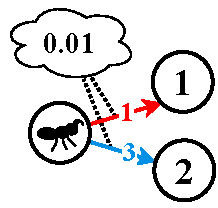
\includegraphics[scale=\scalefigure]{Figures/chap 3/pACO.pdf}
	\caption{An example of an ant find the next move}
	\label{fig:pACO}
\end{figure}

Take the instance in Figure~\ref{fig:individual} as an illustration input of the lower level. Suppose there is an ant that is finding its way to the next node as shown in Figure~\ref{fig:pACO}. In this case, the ant will have to choose one of two paths with the same pheromone trail of 0.01. Therefore, two main factors affecting the ant's path selection include the edge weight and the domain priority of that edge. Assume that the $\alpha, \beta,$ and $\gamma$ are 2, 1, and 2, respectively. The ant will now compute the $P_e$ value of each edge as follows.

\bigskip
$
p_e~red~edge = \frac{0.01^2~\times~(1/1)^1~\times~0.8^2}{(0.01^2~\times~(1/1)^1~\times~0.8^2)~+~(0.01^2~\times~(1/3)^1~\times~0.2^2)} = \frac{48}{49}~\approx0.97
$
\bigskip

$
p_e~blue~edge = \frac{0.01^2~\times~(1/3)^1~\times~0.2^2}{(0.01^2~\times~(1/1)^1~\times~0.8^2)~+~(0.01^2~\times~(1/3)^1~\times~0.2^2)} = \frac{1}{49}~\approx0.02
$ \\ 

It can be seen that the red edge has a higher ant selection rate (0.97 $>$ 0.02) due to its shorter path length and higher domain priority than the blue edge. In this step, Roulette Selection is implemented. Therefore, edges with a low selection rate can still be chosen by ants, which increases the exploitation capability of the colony and avoids falling into the local optima.

\begin{algorithm}
	%\setstretch{0.9}
	\caption{Ant's Pathfinding Algorithm (APA)}
	\label{alg:apa}
	\textbf{Input}:	
	\begin{itemize}
		\item A filtered multi-graph $G' = (V', E', w, s, t)$;
		\item An individual $I = (\pi_1, \pi_2,...,\pi_{|D|})$;
	\end{itemize}
	\textbf{Output}: A path $p = \{s, p_1, \dots, t\}$ and its cost. \\
	\Begin
	{	
		$D_{visited} \leftarrow\emptyset$ \Comment{List of visited domains}\;
		$visited[v] \leftarrow false~\forall v \in V$ \Comment{List of visited nodes}\;
		$cur \leftarrow s$ \Comment{The node that ant $k$ is visiting}\;
		$d \leftarrow  -1$ \Comment{The edge's domain that $p$ is visiting}\;
		\tcc{c(v) is the cost from s to v}
		$c(s) \leftarrow 0$, $c(t) \leftarrow \infty$;\\
		\While{$cur \neq t$}
		{
			$visited[cur] \leftarrow true$\;
			$Adj(cur) \leftarrow$ The set of edges that connect $v$ to other unvisited nodes in $G'$, in which each edge must satisfy the $Checksum$, $Domain~Blacklist~Check$, and its domain is not in $D_{visited}$\;
			%			$Adj(cur) \leftarrow$ Construct set of candidate edges 
			% \Comment{Refer to Algorithm~\ref{alg:edge-set}}\;
			\If{$Adj(cur) = \emptyset$}{ break\;}
			\If{$k$ is dull ant}{
				$e \leftarrow$ Choose an edge based on its attractiveness\;
			}
			\Else{
				Calculate the probability of moving to each edge as Equation (1)\;
				$e \leftarrow$ Choose an edge by $Roulette~Selection$\;
			}
			$d' \leftarrow$ the domain of $e$\;
			\If{$d \neq -1~and~d' \neq d$}{
				$D_{visited} \leftarrow D_{visited} \cup \{d\}$
			}
			$d \leftarrow d'$; $c(v) \leftarrow c(cur) + w(e)$;  $cur \leftarrow v$\; 
		}
		\Return $p$ and $c(t)$\;
	}
\end{algorithm}

In addition, to facilitate the ants’ search process and help ants avoid getting stuck, three components are integrated into the proposed \acrshort{gaco}, which will be discussed in the following subsections.

\subsection{Ant Colony Optimization with Dull Ants}
Typically, traditional \gls{aco} approaches have a potential drawback of premature convergence to a local optimum, often caused by a large amount of pheromone deposited by previous ant generations. Together with minimizing the impact of this phenomenon, a new type of ant, called $dull~ant$~\cite{shimomura2010ant}, is added to the colony. The notable feature of dull ant is that while it can neither trail the pheromone nor perceive the domains' priority, it can still deposit the pheromone. Therefore, dull ants will not be affected by other ants, opening up opportunities to discover alternatively better paths.

\subsection{Checksum}
To ease the search for each ant, a second component is employed, coined $Checksum$. Before choosing an edge $e$, ant $k$ will sum its current path length and the weight of $e$. If this sum is greater than the currently found best solution, $e$ is removed from the candidate edge set. Checksum not only expedites the ant's search process but also ensures that the solution located will always be better than the previous one.
Figure~\ref{fig:checksum} is a typical example of an ant checking the Checksum. Assume that the currently best solution found is 20 and the current path length of the considered ant is 17, and the \gls{du} are still satisfied.The ant will then sum its path value with each edge leading to the subsequent nodes. Following Checksum, the green edge leading to node 4 will be removed from the candidate edge set since $17 + 4 = 21 > 20$.

\setlength{\intextsep}{3pt}
\renewcommand{\scalefigure}{1.1}
\begin{figure}[htbp]
	\centering
	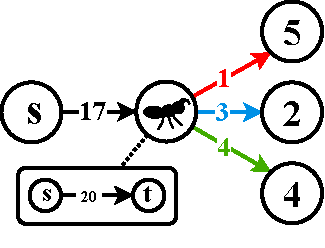
\includegraphics[scale=\scalefigure]{Figures/chap 3/CheckSum.pdf}
	\caption{An example of an ant checking the Checksum}
	\label{fig:checksum}
\end{figure}

\subsection{Blacklist of Domains on each Node}
One problem encountered when applying \gls{aco} to incomplete graphs is that ant gets stuck at a specific node since there is no subsequent path. Moreover, this phenomenon transpires more frequently in \gls{idpcdu}, where ant not only finds a path, but the path must also fulfill the \gls{du} constraint. In other words, a domain sequence is deemed to be stuck when an ant is unable to find any edges satisfying the \gls{du} constraint leading to one of the subsequent nodes. To remedy this shortcoming, an anti-stuck strategy for multi-domain problems like \gls{idpcdu} is proposed as follows. Except for the source and destination, every time an ant arrives at a stuck node, its list of visited domains is stored in the node's blacklist. Before deciding an edge $e$, the ant checks if the edge's domain $d$ is the one that causes a stuck of any sequence of domains in the blacklist of the node to which it leads. In such a case, the ant will continue to scan whether its list of visited domains is a superset of the other after discarding $d$. Consequently, $d$ will be removed from the candidate edge set if this point is satisfied. Algorithm~\ref{alg:blacklist} presents how to check if a list of domains is in the blacklist of any node. Note that before being saved to the blacklist as well as when the ant performs the $Domain~Blacklist~Check$, the domains will be sorted in a particular predefined order. Thus, the retrieval of data is performed faster, saving both time and resources.

\bigskip
\begin{algorithm}
	%\setstretch{0.9}
	\caption{Domain Blacklist Check}
	\label{alg:blacklist}
	\textbf{Input}:	
	\begin{itemize}
		\item A list of domains $LD$;\\
		\item A blacklist $blacklist^v$ of node $v$;\\
	\end{itemize}
	\textbf{Output}: $LD$ is in $blacklist^v$ or not.\\
	\Begin
	{	
		$d \leftarrow $ the last element in $LD$\;
		$LD' \leftarrow LD$ without $d$\;		
		\ForEach{list of domains $LD_i$ in $blacklist^v$}
		{
			$d_i \leftarrow $ the last element in $LD_i$\;
			\If{$d = d_i$}
			{
				$LD_i' \leftarrow LD_i$ without $d_i$\;
				\If{$LD_i' \subseteq LD'$} {\Return true\;}
			}
		}
		\Return false\;
	}
\end{algorithm}
\bigskip
\setlength{\intextsep}{3pt}
\renewcommand{\scalefigure}{1}
\begin{figure}[htbp]
	\centering
	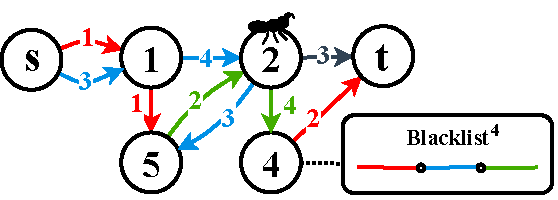
\includegraphics[scale=\scalefigure]{Figures/chap 3/BlacklistV2.pdf}
	\caption{An example of an ant checking the blacklist}
	\label{fig:blacklist}
\end{figure}
\bigskip
Take Figure~\ref{fig:blacklist} as a sample blacklist implementation in ant's route selection. Suppose that the blacklists of all nodes are initially empty, and an edge that goes from node $i$ to $j$ with an associated weight $w$ and belongs to domain $d$ is denoted by $(i, j, w, d)$. The first ant starts from $(s, 1, 1, red)$, $(1, 2, 4, blue)$, $(2, 4, 4, green)$ and gets stuck at node 4 because it can only revisit the $red$ domain. Therefore, the order of domains $(red, blue, green)$ is added to the blacklist of node 4. The next ant has the same beginning as the previous one. When standing at node 2, it realizes that there is only one route $(2, 4, 4, green)$, which also belongs to the domain that caused the stuck at node 4. The ant then resumes checking and finds that its visited domains list is also the stuck list without the $green$ domain. Therefore, the ant will remove this edge from the candidate set and select another. An ant has the following path $(s, 1, 3, blue)$, $(1, 5, 1, red)$, $(5, 2, 2, green)$. When it reaches node 2, it does the same thing as the second ant. In this case, its traversed domains list is a superset of the one after discarding the $green$ domain, and in the end, the edge $(2, 4, 4, green)$ is still eliminated. This strategy allows the searching candidate edge of ant more thoroughly without saving a plethora of stuck cases. The shorter the order of domains in blacklists, the more effective this method will be.

\section{Node-defined Domain - A variant of IDPC-DU}
\label{proposed:ndu}
As mentioned above, \acrshort{idpcndu}, which has also been proven to be NP-complete~\cite{maggi2018domain}, is a variant of the original \gls{idpcdu}. In general, previous approaches for \gls{idpcdu} or \acrshort{idpcndu} are often unable, or they have to go through several transformation steps to solve the remaining one. Our proposed algorithm, on the other hand, can be applied to both problems. Since \acrshort{idpcndu} no longer assigns domains on edges, there is only one edge with the smallest weight between any two nodes~\cite{binh2021two}. Therefore, $P_e$ in Equation~\ref{equation:edge_pick} is the domain's priority of the node to which edge $e$ leads. $Adj(v_i)$ now includes all nodes that ant $k$ has not yet traversed, whose domains satisfy the \gls{du} and $Domain~Blacklist~Check$, and the edges directing to these nodes fulfill the $Checksum$.
\chapter{Experimental results}
\label{chap:chap4}
This chapter presents and analyzes the effectiveness of the proposed algorithm on various datasets and compares it with the previous best approaches of \gls{idpcdu}. Details about the evaluation criteria, how to conduct experiments, comparisons, and analyzes will be elaborated.

\section{Problem instances}
\label{experiment:dataset}
To evaluate the performance of the proposed \acrshort{gaco}, 
this thesis utilize the public dataset generated in~\cite{binh2020multifactorial} for \gls{idpcdu} to evaluate the performance of the proposed \acrshort{gaco}. 

This dataset is constructed as follows. Firstly, each dataset will have three input parameters, including the number of nodes, the number of domains, and the number of edges. Secondly, an array of nodes and an array of domains are initialized separately such that the number of nodes must be greater than the number of domains. The source and destination nodes are set at the start and end of the node array, respectively. Next, from two pre-made arrays, the shortest path $p$, which is also the solution of the dataset, is created. Each edge of $p$ is assigned a weight of 1, except for the outgoing edge of the source node which is set to a weight of 2. Then the dataset is added noises to prevent simple greedy algorithms from brute-force searching for the optimal solution effortlessly. For each node in $p$, edges with random weights that lead to ones other than those in $p$ will be randomly added, especially as there is bound to be an edge with a weight of 1. Finally, the edge with a weight greater than the value of edges in $p$ is initialized on the remaining nodes of the array. This method of generating datasets ensures that $p$ is the global optimal of that dataset.

%The dataset consists of a small set with nodes ranging from 10 to 45 and a large group with 50 to 100.
This dataset comprises two sets of instances, including a small set, where the number of nodes ranges from 10 to 45 with an increment of 5, and a large one, where the number of nodes varies from 50 to 100 with an increment of 10.
The number of domains corresponding to each instance is generated by multiplying the number of nodes by a ratio of 0.5, 1.0, and 2.0. Details of the dataset are available in~\cite{idpcdu2020data}.

\section{Experimental criteria}
\label{experiment:criteria}
Table~\ref{tab:criteria} lists the criteria for evaluating the quality of the algorithms.
\bigskip
\begin{table}[htbp]
	\centering
	\caption{Criteria for evaluating the quality of algorithms}
	\scalebox{1}{
		\begin{tabular}{ll}
			\toprule
			AVG & The average function value over all runs \\
			BF & The best function value found over all runs\\
			STD & Standard Deviation \\
			RPD & Relative Percentage Differences\\
			PI & Improvement Percentage  \\
			\bottomrule
		\end{tabular}
	}
	\label{tab:criteria}
\end{table}
\bigskip
Let $S^i_{ar}$ be the solution provided by the considered algorithm $a$, for instance $i$, on the $r$-th run. Let $B^i$ be the best solution obtained among all algorithms for $i$. For minimization problems, the \gls{rpd} is calculated using Equation~\ref{equa:rpd}. The smaller the \gls{rpd} value, the better the quality of the solution found.
\begin{equation}
	\label{equa:rpd}
	{RPD}^i_{ar} = \frac{S^i_{ar} - B^i}{B^i} \times 100
\end{equation}

The \gls{pi} is also often used to compare two algorithms $a$ and $b$. Let $AVG^i_a$ and $AVG^i_b$ be the average function values given by $a$ and $b$ on $i$, respectively. The \gls{pi} of $a$ compared to $b$ on $i$ is then computed as Equation~\ref{equa:pi}. On the other hand, the greater the \gls{pi}, the larger the considered algorithm's improvement.
\begin{equation}
	\label{equa:pi}
	{PI}^i_{ab} = \frac{{AVG}^i_a - {AVG}^i_b}{{AVG}^i_b} \times 100
\end{equation}

\section{Experimental setups}
\label{experiment:setup}
To reveal the strengths and weaknesses of \acrshort{gaco}, this paper adopted the \gls{mfea} proposed in~\cite{binh2020multifactorial}, named \acrshort{mfea-edu}, and an \gls{saco} algorithm introduced in~\cite{sudholt2012simple}, as comparison algorithms. The efficiency of this multitasking algorithm compared to single-tasking one had been confirmed experimentally. Thus, we reuse the same parameters as in the original paper to create a similar experimental environment, thereby maximizing the performance of \acrshort{mfea-edu}. 
For \acrshort{saco}, its parameters are also used as in the original study, except for $\alpha,~\beta,$ and $Q$, which are taken from the \gls{aco} level in \acrshort{gaco}.
Turning to the proposed algorithm, based on preliminary experiments, we observed that a parameter set used for the \gls{aco} level achieved the best performance on the dataset. Thus, it is employed in the following experiments. Table~\ref{tab:paramGACO} shows all parameters used in \acrshort{gaco}.

Besides, each algorithm was simulated 30 times on the same computer (Intel Core i7 - 3.60GHz, 16GB RAM) with the total number of task evaluations is 50000. The source codes were installed in Java language.
\bigskip
\begin{table}[H]
	\centering
	\caption{The parameter set used for \acrshort{gaco}}
	\scalebox{1}{
		\begin{tabular}{clc}
			\toprule
			& \multicolumn{1}{c}{\textbf{Parameter Name}} & \multicolumn{1}{c}{\textbf{Parameter Value}}\\
			\midrule
			\parbox[t]{2mm}{\multirow{4}{*}{\rotatebox[origin=c]{90}{\textbf{\gls{ga}}}}} & Population Size ($N$) & 25\\
			& Number of generations ($GEN\_GA$) & 20\\
			& Crossover Rate (pc) & 0.5\\
			& Mutation Rate (pm) & 0.05\\
			\midrule
			\parbox[t]{2mm}{\multirow{4}{*}{\rotatebox[origin=c]{90}{\textbf{\gls{aco}}}}} & Population Size ($M$) & 20\\
			& Number of $dull~ants$ & M*20$\% $ \\
			& Number of generations ($GEN\_ACO$) & 5\\
			& $\alpha,~\beta,~\gamma,~Q$ & 3, 5, 5, 5\\
			\bottomrule
		\end{tabular}
	}
	\label{tab:paramGACO}
\end{table}

\section{Experimental results}
\label{experiment:result}
The performance of \acrshort{gaco} for \gls{idpcdu} is evaluated under three analyses:
\begin{itemize}
	\item Analysis of the algorithm's computational complexity.
	\item Analysis of the obtained results by the Non-parametric statistic.
	\item Analysis quality of the proposed algorithm in comparison with other algorithms.
\end{itemize}

\subsection{Analysis of the algorithm's computational complexity}
The number of times \acrshort{gaco} is iterated is denoted by $GEN\_GA$. In each iteration, the execution times of the crossover, mutation, and decoding operators are $N, p_m * N$, and $N$ times, respectively. The complexity of the algorithm is as follows:
$O($\acrshort{gaco}$)$ = $O($Pre-filtering process$)$ + $O($Initialization$)$ + $GEN\_GA\times \bigg(N \times O($Crossover$)$ + $p_{m}\times N\times O($Mutation$)$ + $N\times O($Evaluation$)$ + $O($Selection$)\bigg)$, in which the complexity of each component is as follows:
\begin{itemize}
	\item In the pre-filtering process, each edge in $G$ is traversed  one time. Therefore, the complexity of the pre-filtering process is $O(|E|)$, with $|E|$ being the number of edges in the initial graph.
	\item The initialization method needs a computational cost $O(|D|\times N)$ to generate $N$ random individuals, with $|D|$ being the number of domains.
	\item The complexity of mutation, crossover, and survival selection operators are $O(1)$, $O(|D|)$, and $O(NlogN)$, respectively.
	\item The fitness evaluation uses \gls{aco} algorithm, which starts with the initial pheromone on all edges of $G'$, so the running time of this process is $O(|E'|)$. Then, \gls{aco} performs $GEN\_ACO$ iterations over the following steps: construct solutions for $M$ ants and updates pheromone. A solution is built by Algorithm~\ref{alg:apa} with a running time of $O(|E'|\times |D|^2)$. Because each ant travels through nodes on $G'$, it constructs a list of candidate adjacent edges at every visited node. Each edge is added to the list with the running time of $O(|1|)$ of checking the $Checksum$ and $O(|D|^2)$ of the $Domain~Blacklist~Check$. Besides, every candidate list of adjacent edges has its size no more than the out-degree of the currently visited, and the total out-degree of all nodes on $G'$ is the number of edges. Update pheromone has a running time of $O(|V'|)$ because the maximum path length is the number of nodes on $G'$. Therefore, the computational complexity of the \gls{aco} algorithm is $O(ACO\;initialization)\;+\;GEN\_ACO\times M\times (O(ACO\;construct\;solutions)\;+\;O(ACO\;update\;pheromone))$, in which the complexity of \gls{aco} initialization, construct solutions, and update pheromone are $O(|E'|)$, $O(|E'|\times |D|^2)$, and $O(|V'|)$.
\end{itemize}
Therefore, $O($\acrshort{gaco}$) = $
$O(|E|) + O(|D|\times N)$ + $GEN\_GA\times\bigg(N \times O(|D|) + p_{m}\times N\times O(1) + N\times GEN\_ACO\times (O(|E'|) + M\times (O(|E'|)\times (O(1)+O(|D|^2)))) + N\times O(logN))\bigg)$
= $O\bigg(GEN\_GA\times N\times (GEN\_ACO\times M\times|E'|\times|D|^2 +logN)\bigg)$.

\subsection{Analysis of the obtained results by the Non-parametric statistic}
The Non-parametric statistic is used to compare the effectiveness of the following algorithms: \acrshort{saco}, \acrshort{mfea-edu}, and the proposed \acrshort{gaco}. The process of comparison involves two significant steps:
\begin{itemize}
	\item First, statistical approaches such as Friedman, Aligned Friedman, and Quade~\cite{carrasco_recent_2020, derrac_practical_2011} are used to evaluate the differences among results obtained by the above algorithms.
	\item After rejecting the hypothesis of equivalent means for the results obtained by the algorithms in the first step, post-hoc statistical procedures~\cite{carrasco_recent_2020} are employed to compute the concrete differences between the algorithms and compare a control algorithm to the remaining algorithms.
\end{itemize}

Tables~\ref{tab:type_1} and \ref{tab:type_2} show the results of algorithms on different types of instances. The red, black, and blue cells in a column of \acrshort{gaco} in these tables denote instances where this algorithm is better, equal, and worse than the others.
The results of Friedman's and Iman-Davenport's tests are shown in Table~\ref{tab:Results_Friedman}. As seen in the table, every Friedman and Iman-Davenport value surpasses the critical value. In addition, all $p$-values are less than 0.05, so all the null hypotheses, i.e., the equivalence of the medians of the results of the different benchmarks, are rejected. In other words, there are significant differences among the observed results with a probability error of $p \leq 0.05$. Table~\ref{tab:Results_Rank} illustrates the rankings achieved by the Friedman, Friedman Aligned, and Quade tests. The results in this table strongly indicate considerable differences between the algorithms.

\begin{table}
	\centering
	\caption{Results of the Friedman and Iman-Davenport test ($\alpha$=0.05)}
	\label{tab:Results_Friedman}
	\scalebox{1}{
		\begin{tabular}{c c c c c c}
			\toprule
			Friedman Value & Value in $X^2$ & $p$-value \\
			\cmidrule(l{3pt}r{3pt}){1-3} 
			\textbf{60.250} & 5.991 & $6.942*10^{-11}$ \\ 
			\addlinespace
			\midrule
			Iman-Davenport Value & Value in $F_F$ & $p$-value \\
			\cmidrule(l{3pt}r{3pt}){1-3}
			\textbf{104.010} & 3.107 & $3.211*10^{-23}$\\
			\bottomrule
		\end{tabular}
	}
\end{table}

\begin{table}
	\centering
	\caption{Average rankings achiedved by the Friedman, Friedman Aligned, and Quade tests}\label{tab:Results_Rank}
	\scalebox{1}{
		\begin{tabular}{c c c c}
			\toprule
			Algorithms & Friedman & Friedman Aligned & Quade \\
			\midrule
			\acrshort{saco} & 2.773 & 90.940 & 2.835 \\
			\acrshort{mfea-edu} & 2.130 & 77.154 & 2.146 \\
			\acrshort{gaco} & 1.095 & 22.404 & 1.018 \\
			\bottomrule
		\end{tabular}
	}
\end{table}

\begin{table}[!htp]
	\centering
	\caption{The z-values and p-values of the Friedman procedures (\glsentrytext{gaco} is the control algorithm)} 
	\label{tab:CompareControlAlg}
	\scalebox{1}{
		\begin{tabular}{cc cccc}
			\toprule
			& & \multicolumn{4}{c}{\textbf{Friedman}} \\
			\cmidrule(l{3pt}r{3pt}){1-2}
			\cmidrule(l{3pt}r{3pt}){3-6}
			$i$ & 
			Algorithms &
			$z$ &
			$p$ &
			Holm &
			Holland \\
			\midrule
			2 & \acrshort{saco} & 7.69 & $1.44*10^{-14}$ & 0.025 & 0.025\\
			1 & \acrshort{mfea-edu} & 4.74  & $2.07*10^{-6}$ & 0.05 & 0.05\\
			\bottomrule
		\end{tabular}
	}
\end{table}

Table~\ref{tab:Results_Rank} also point out that the \acrshort{gaco} has the smallest ranking; thus, it is selected as the control algorithm. After that, we compare the control algorithm with two other ones (\acrshort{mfea-edu} and \acrshort{saco}) by using more powerful statistical methods, i.e., Holland and Holm. Table~\ref{tab:CompareControlAlg} shows all the possible hypotheses of comparison between the control algorithm and other algorithms, ordered by their $p$-value and associated with their level of significance. A common highlight from table~\ref{tab:Results_Friedman} is that the control algorithm outperforms \acrshort{saco} and \acrshort{mfea-edu} with a level of significance $\alpha = 0.05$.

\renewcommand{\scalefigure}{0.5}
\begin{figure}[htbp]
	\centering
	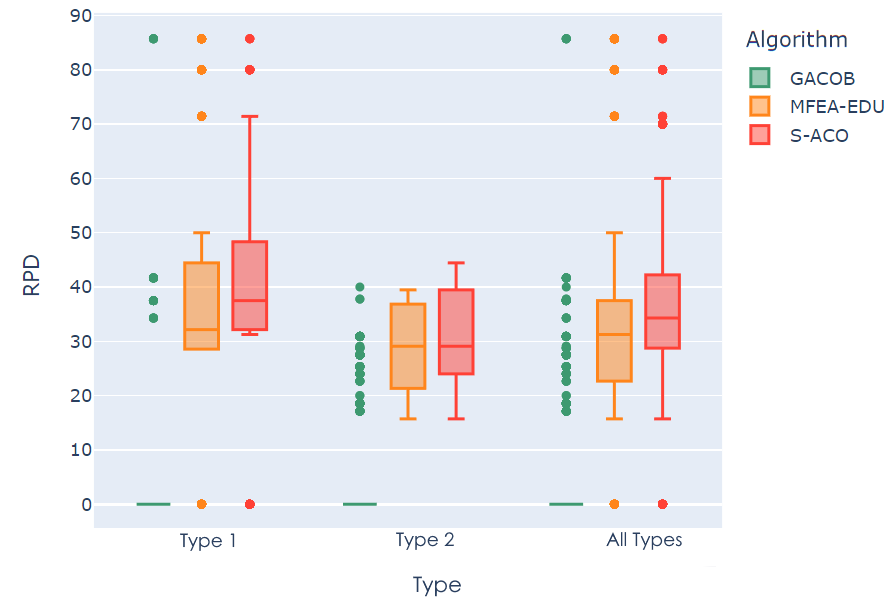
\includegraphics[scale=\scalefigure]{Figures/chap 4/RPD_each_set.png}
	\caption{The obtained RPD values of all algorithms}
	\label{fig:rpd}
\end{figure}

\subsection{Analysis quality of the proposed algorithm in comparison with other algorithms}
The experimental results shown in Table~\ref{tab:type_1} and Table~\ref{tab:type_2} have pointed out that \acrshort{gaco} outperforms \acrshort{saco} and \acrshort{mfea-edu} on both the best value, average, and standard deviation in most instances, except small instant Idpc\_10x10x1000. The box and whisker plots of each instance type and the three algorithms (\acrshort{gaco}, \acrshort{mfea-edu}, and \acrshort{saco}) are shown in Figure~\ref{fig:rpd}. Our algorithm finds the best solution every time, which is why the box and whisker plots in Type 1, Type 2, and All Types are reduced to single lines. The average \gls{pi} of \acrshort{gaco} compared to \acrshort{saco}, as shown in Table~\ref{tab:pi}, is 24.6\% in Type 1 and  18.7\% in Type 2. Meanwhile, the percentage for \acrshort{mfea-edu} is 21.0\% in Type 1 and 17.4\% in Type 2. Overall, the proposed \acrshort{gaco} improves \acrshort{mfea-edu}  19.4\% in terms of the average result, and the enormous gap recorded is 44.4\%.

\begin{table}[htbp]
	\centering
	\caption{The PI of \acrshort{gaco} compared to other algorithms}
	\scalebox{0.9}{
		\begin{tabular}{clccccccc}
			\toprule
			\multirow{2}[4]{*}{} & \multicolumn{1}{l}{\multirow{2}[4]{*}{\textbf{Type}}} & \multicolumn{3}{c}{\textbf{GACOB - S-ACO}} & & \multicolumn{3}{c}{\textbf{GACOB - MFEA-EDU}}  \\
			\cmidrule{3-5} \cmidrule{7-9}& & \textbf{MIN PI} & \textbf{AVG PI} & \textbf{MAX PI} & & \textbf{MIN PI} & \textbf{AVG PI} & \textbf{MAX PI} \\
			\midrule
			& Type 1 & -2.6 & 24.6 & 39.1  & & -1.0 & 21.0 & 44.4\\
			& Type 2 & 2.4  & 18.7 & 29.4 & & 0.2 & 17.4 & 28.3 \\
			\midrule
			& All instances & -2.6  & 22.1 & 39.1 & & -1.0 & 19.4 & 44.4 \\
			\bottomrule
		\end{tabular}%
	}
	\label{tab:pi}%
\end{table}%

\begin{table}[htbp]
	\centering
	\caption{The obtained results of all algorithms in Type 1}
	\scalebox{0.9}{
		\begin{tabular}{clccccccccccc}
			\toprule
			\multirow{2}[4]{*}{} & \multicolumn{1}{l}{\multirow{2}[4]{*}{\textbf{Instances}}} & \multicolumn{3}{c}{\textbf{S-ACO}} & & \multicolumn{3}{c}{\textbf{MFEA-EDU}} & & \multicolumn{3}{c}{\textbf{GACOB}}  \\
			\cmidrule{3-5} \cmidrule{7-9} \cmidrule{11-13}& & \textbf{BF} & \textbf{AVG} & \multicolumn{1}{p{2.5em}}{\textbf{STD}} & & \textbf{BF} & \textbf{AVG} & \multicolumn{1}{p{2.5em}}{\textbf{STD}} & & \textbf{BF} & \textbf{AVG} & \multicolumn{1}{p{2.5em}}{\textbf{STD}} \\
			\midrule
			& Idpc\_10x10x1000 & 7  & 7.80  & 2.07 & & 7 & 12.20 & 2.07  & & 7 & \textcolor[rgb]{ 0,  0,  1}{8.00} & 2.27  \\
			& Idpc\_10x20x2713 & 7  & 7.83  & 1.90 & & 12 & 12.00 & 0.00  & & 7 & \textcolor[rgb]{ 1,  0,  0}{7.00} & 0.00 \\
			& Idpc\_10x5x425 & 7  & 7.00  & 0.00 & & 7 & 7.00 & 0.00  & & 7 & \textcolor[rgb]{ 0,  0,  0}{7.00} & 0.00 \\
			& Idpc\_15x15x3375 & 16  & 16.40  & 0.50 & & 10 & 10.00 & 0.00  & & 10 & \textcolor[rgb]{ 0,  0,  0}{10.00} & 0.00 \\
			& Idpc\_15x30x12111 & 10  & 16.43  & 1.30 & & 10 & 10.00 & 0.00  & & 10 & \textcolor[rgb]{ 0,  0,  0}{10.00} & 0.00 \\
			& Idpc\_15x7x1504 & 10  & 13.73  & 4.06 & & 18 & 18.00 & 0.00  & & 10 & \textcolor[rgb]{ 1,  0,  0}{10.00} & 0.00 \\
			& Idpc\_20x10x2492 & 22  & 22.00  & 0.00 & & 22 & 22.00 & 0.00  & & 15 & \textcolor[rgb]{ 1,  0,  0}{15.00} & 0.00 \\
			& Idpc\_20x20x8000 & 21  & 22.07  & 0.83 & & 15 & 15.40 & 1.52  & & 15 & \textcolor[rgb]{ 1,  0,  0}{15.00} & 0.00 \\
			& Idpc\_20x40x26104 & 21  & 22.00  & 0.37 & & 15 & 15.20 & 1.10  & & 15 & \textcolor[rgb]{ 1,  0,  0}{15.00} & 0.00 \\
			& Idpc\_25x12x4817 & 27  & 27.00  & 0.00 & & 27 & 27.00 & 0.00  & & 18 & \textcolor[rgb]{ 1,  0,  0}{18.00} & 0.00 \\
			& Idpc\_25x25x15625 & 26  & 26.90  & 0.31 & & 18 & 24.13 & 3.44  & & 18 & \textcolor[rgb]{ 1,  0,  0}{18.00} & 0.00 \\
			& Idpc\_20x50x57147 & 26  & 26.93  & 0.25 & & 18 & 24.67 & 3.03  & & 18 & \textcolor[rgb]{ 1,  0,  0}{18.00} & 0.00 \\
			& Idpc\_30x15x10025 & 33  & 33.93  & 0.25 & & 33 & 33.00 & 0.00 & & 33 & \textcolor[rgb]{ 1,  0,  0}{33.33} & 0.48 \\
			& Idpc\_30x30x27000 & 32  & 32.73  & 0.45 & & 32 & 32.00 & 0.00 & & 24 & \textcolor[rgb]{ 1,  0,  0}{24.00} & 0.00 \\
			& Idpc\_30x60x89772 & 32  & 32.33  & 0.48 & & 32 & 32.00 & 0.00 & & 24 & \textcolor[rgb]{ 1,  0,  0}{24.00} & 0.00 \\
			& Idpc\_35x17x13934 & 38  & 38.50  & 0.51 & & 38 & 38.00 & 0.00 & & 28 & \textcolor[rgb]{ 1,  0,  0}{28.00} & 0.00 \\
			& Idpc\_35x35x42875 & 37  & 38.47  & 0.82 & & 37 & 37.00 & 0.00 & & 28 & \textcolor[rgb]{ 1,  0,  0}{28.00} & 0.00 \\
			& Idpc\_35x70x123585 & 37  & 37.00  & 0.00 & & 28 & 35.47 & 2.03 & & 28 & \textcolor[rgb]{ 1,  0,  0}{28.00} & 0.00 \\
			& Idpc\_40x20x18485 & 42  & 42.97  & 0.18 & & 42 & 42.00 & 0.00 & & 32 & \textcolor[rgb]{ 1,  0,  0}{32.00} & 0.00 \\
			& Idpc\_40x40x64000 & 42  & 42.00  & 0.00 & & 42 & 42.00 & 0.00 & & 32 & \textcolor[rgb]{ 1,  0,  0}{32.00} & 0.00 \\
			& Idpc\_40x80x130681 & 42  & 42.00  & 0.00 & & 42 & 42.00 & 0.00 & & 32 & \textcolor[rgb]{ 1,  0,  0}{32.00} & 0.00 \\
			& Idpc\_45x22x43769 & 47  & 47.00  & 0.00 & & 47 & 47.00 & 0.00 & & 35 & \textcolor[rgb]{ 1,  0,  0}{37.00} & 4.55 \\
			& Idpc\_45x45x91125 & 47  & 48.93  & 0.37 & & 46 & 46.00 & 0.00 & & 35 & \textcolor[rgb]{ 1,  0,  0}{35.00} & 0.00 \\
			& Idpc\_45x90x322081 & 46  & 46.90  & 0.31 & & 46 & 46.00 & 0.00 & & 35 & \textcolor[rgb]{ 1,  0,  0}{35.00} & 0.00 \\
			\bottomrule
		\end{tabular}
	}
	\label{tab:type_1}%
\end{table}

\begin{table}[htbp]
	\centering
	\caption{The obtained results of all algorithms in Type 2}
	\scalebox{0.9}{
		\begin{tabular}{clccccccccccc}
			\toprule
			\multirow{2}[4]{*}{} & \multicolumn{1}{l}{\multirow{2}[4]{*}{\textbf{Instances}}} & \multicolumn{3}{c}{\textbf{S-ACO}} & & \multicolumn{3}{c}{\textbf{MFEA-EDU}} & & \multicolumn{3}{c}{\textbf{GACOB}}  \\
			\cmidrule{3-5} \cmidrule{7-9} \cmidrule{11-13}& & \textbf{BF} & \textbf{AVG} & \multicolumn{1}{p{2.5em}}{\textbf{STD}} & & \textbf{BF} & \textbf{AVG} & \multicolumn{1}{p{2.5em}}{\textbf{STD}} & & \textbf{BF} & \textbf{AVG} & \multicolumn{1}{p{2.5em}}{\textbf{STD}} \\
			\midrule
			& Idpc\_100x100x1000000 & 103  & 103.03  & 0.18  & & 102 & 102.00 & 0.00  & & 80 & \textcolor[rgb]{ 1,  0,  0}{91.17} & 11.36  \\
			& Idpc\_100x200x2296097 & 102  & 102.00  & 0.00 & & 101 & 101.00 & 0.00  & & 80 & \textcolor[rgb]{ 1,  0,  0}{96.87} & 9.46 \\
			& Idpc\_100x50x461319 & 103  & 103.00  & 0.00 & & 102 & 102.07 & 0.37  & & 80 & \textcolor[rgb]{ 1,  0,  0}{80.00} & 0.00 \\
			& Idpc\_50x100x285357 & 52  & 52.00  & 0.00 & & 52 & 52.00 & 0.00  & & 38 & \textcolor[rgb]{ 1,  0,  0}{38.00} & 0.00 \\
			& Idpc\_50x25x38961 & 53  & 53.00  & 0.00 & & 53 & 53.00 & 0.00  & & 38 & \textcolor[rgb]{ 1,  0,  0}{38.00} & 0.00 \\
			& Idpc\_50x50x125000 & 53  & 53.00  & 0.00 & & 52 & 52.00 & 0.00  & & 38 & \textcolor[rgb]{ 1,  0,  0}{38.00} & 0.00 \\
			& Idpc\_60x120x434337 & 64  & 64.07  & 0.25 & & 61 & 61.00 & 0.00  & & 45 & \textcolor[rgb]{ 1,  0,  0}{45.60} & 3.29 \\
			& Idpc\_60x30x99470 & 62  & 63.93  & 0.37 & & 62 & 62.00 & 0.00  & & 45 & \textcolor[rgb]{ 1,  0,  0}{46.13} & 4.31 \\
			& Idpc\_60x60x216000 & 62  & 63.73  & 0.58 & & 62 & 62.00 & 0.00  & & 45 & \textcolor[rgb]{ 1,  0,  0}{45.00} & 0.00 \\
			& Idpc\_70x140x923343 & 73  & 73.00  & 0.00 & & 72 & 72.00 & 0.00  & & 55 & \textcolor[rgb]{ 1,  0,  0}{66.90} & 7.92 \\
			& Idpc\_70x35x120810 & 72  & 72.97  & 0.18 & & 72 & 72.00 & 0.00  & & 55 & \textcolor[rgb]{ 1,  0,  0}{55.57} & 3.10 \\
			& Idpc\_70x70x343000 & 71  & 72.73  & 0.64 & & 71 & 71.00 & 0.00  & & 55 & \textcolor[rgb]{ 1,  0,  0}{56.07} & 4.06 \\
			& Idpc\_80x160x1490468 & 81  & 81.93 & 0.25 & & 81 & 81.00 & 0.00  & & 70 & \textcolor[rgb]{ 1,  0,  0}{70.00} & 0.00 \\
			& Idpc\_80x40x175762 & 82  & 82.97  & 0.18 & & 82 & 82.00 & 0.00  & & 70 & \textcolor[rgb]{ 1,  0,  0}{70.80} & 3.04 \\
			& Idpc\_80x80x512000 & 82  & 83.87 & 0.43 & & 82 & 82.00 & 0.00  & & 70 & \textcolor[rgb]{ 1,  0,  0}{81.83} & 3.27 \\
			& Idpc\_90x180x1644367 & 92 & 92.00 & 0.00 & & 91 & 91.00 & 0.00  & & 75 & \textcolor[rgb]{ 1,  0,  0}{77.83} & 6.44 \\
			& Idpc\_90x45x260195 & 93 & 93.00 & 0.00 & & 93 & 93.20 & 0.48  & & 75 & \textcolor[rgb]{ 1,  0,  0}{75.00} & 0.00 \\
			& Idpc\_90x90x729000 & 93 & 93.97 & 0.18 & & 91 & 91.00 & 0.00 & & 75 & \textcolor[rgb]{ 1,  0,  0}{87.97} & 8.64 \\
			\bottomrule
		\end{tabular}%
	}
	\label{tab:type_2}%
\end{table}




\chapter*{Conclusion}
\addcontentsline{toc}{chapter}{Conclusion}
This thesis introduces a two-level strategy termed \acrshort{gaco}, which combines two metaheuristic algorithms, namely \gls{ga} and \gls{aco}, to grapple with both variants of \gls{idpcdu}. In the proposed algorithm, a prefiltering process and a new chromosome encoding method that decreases the chromosome length to the number of domains are also integrated. Furthermore, \acrshort{gaco} is armed with an anti-stuck mechanism that helps ants avoid being stuck, which is an inherent problem when applying this algorithm to directed graph problems. In order to analyze the proposal’s efficacy, experiments and comparisons with several algorithms on various-sized data sets were conducted. The computational results demonstrated that \acrshort{gaco} outperforms other compared algorithms in virtually all cases.

Specifically, the contributions of this thesis can be summarized as follows:
\begin{itemize}
	\item Propose a two-level algorithm combining \gls{ga} and an improved \gls{aco} to solve \gls{idpcdu}.
	\item Devise an anti-stuck strategy for ants when applying \gls{aco} to multi-domain network problems, such as \gls{idpcdu}.
	\item Conduct experiments on various test instances and comparison with several previous approaches to prove the efficiency of the proposed model.
\end{itemize}

On the other hand, the proposed algorithm still possesses several limitations. The first one to mention is the long-running time of the algorithm. The cause of this can be due to the pre-filtering process combined with the ant pathfinding. However, this is also a trade-off. Although the running time is a bit long, the results of the proposed algorithm have been proven by experiments, which outperform the compared algorithms in most cases. The second limitation is that this thesis only contains experiments in solving the \gls{idpcedu}, even though the proposed algorithm can be applied to solve both versions of this problem.

In general, \gls{idpcdu} can be applied not only in the network field but also in many other ones such as transportation and military. Therefore, it is worth researching deeper on this topic. In the future, this thesis will improve the performance of the proposed algorithm, as well as investigate more about other advanced approaches for \gls{idpcdu}.

A part of the thesis's results has been accepted at the IEEE World Congress on Computational Intelligence (WCCI) 2022 and IEEE Congress on Evolutionary Computation (CEC) 2021:
\begin{itemize}
	\item Do Tuan Anh, \textbf{Nguyen Hoang Long}, Tran Van Diep, and Huynh Thi Thanh Binh,``A Genetic Ant Colony Optimization Algorithm for Inter-domain Path Computation problem under the Domain Uniqueness constraint" in \textit{2022 IEEE World Congress on Computational Intelligence (WCCI)}. (accepted)
	\item Do Tuan Anh, Huynh Thi Thanh Binh, \textbf{Nguyen Hoang Long}, Ta Bao Thang, Su Simon, ``A Two-level Genetic Algorithm for Inter-domain Path Computation under Node-defined Domain Uniqueness Constraints" in \textit{2021 IEEE Congress on Evolutionary Computation (CEC)}. IEEE, 2021, pp. 1–8.
\end{itemize}


\addcontentsline{toc}{chapter}{References} 
\bibliographystyle{IEEEtran}
\bibliography{ref}




\chapter*{Appendix}
\addcontentsline{toc}{chapter}{Appendix}



\end{document}
